%============================================================
%  Capitolo 17 – Advanced Multi-Head Attention
%============================================================
\chapter{Advanced Multi-Head Attention}
\label{ch:advanced-attention}

I modelli linguistici di grandi dimensioni (\emph{Large Language Models}, LLM)
basati su Transformer generano token in modo \textbf{autoregressivo}: ad ogni
passo $t$ viene prodotto un singolo token, dato tutti quelli precedenti.
L'operazione di Self-Attention domina il costo computazionale e di memoria
di questa fase di inferenza. In questo capitolo vengono analizzate le
principali ottimizzazioni architetturali sviluppate per ridurre il costo
della memoria e migliorare l'efficienza dell'inferenza, mantenendo al
contempo una qualità del modello comparabile o superiore alla Multi-Head
Attention standard \citep{vaswani2017attention,bishop2024}.

%------------------------------------------------------------
\section{KV Cache}
\label{sec:kv-cache}

\subsection{Riepilogo della Multi-Head Attention}
\label{subsec:mha-recap}

Nella Multi-Head Attention (MHA) standard, dati i vettori di input
$\mathbf{x}_1, \ldots, \mathbf{x}_s \in \mathbb{R}^{d_{\text{model}}}$
(con $s$ lunghezza della sequenza), per ciascun head $i = 1,\ldots,n$ vengono
calcolate le proiezioni:
\begin{align}
  Q_i &= X W_Q^{(i)}, \quad K_i = X W_K^{(i)}, \quad V_i = X W_V^{(i)},
\end{align}
dove $X \in \mathbb{R}^{s \times d_{\text{model}}}$ è la matrice degli
embedding di input e $W_Q^{(i)}, W_K^{(i)}, W_V^{(i)} \in
\mathbb{R}^{d_{\text{model}} \times d_h}$ sono le matrici di proiezione del
$i$-esimo head, con $d_h = d_{\text{model}} / n$ dimensione del singolo head.

Il punteggio di attenzione per il head $i$ è:
\begin{equation}
  \text{Attention}(Q_i, K_i, V_i) = \text{Softmax}\!\left(
    \frac{Q_i K_i^\top}{\sqrt{d_h}}
  \right) V_i.
  \label{eq:sdpa}
\end{equation}
Le uscite di tutti gli head vengono concatenate e proiettate:
\begin{equation}
  \text{MHA}(X) = \bigl[\text{head}_1;\ldots;\text{head}_n\bigr] W_O,
  \qquad W_O \in \mathbb{R}^{d_{\text{model}} \times d_{\text{model}}}.
\end{equation}
Nell'attenzione \textbf{mascherata} (causale), utilizzata nei modelli decoder,
la matrice di attenzione è una matrice triangolare inferiore: il token in
posizione $t$ può attendere solo ai token nelle posizioni $1, \ldots, t$,
impedendo la visione anticipata dei token futuri.

\subsection{Computazione a ogni passo autoregressivo}
\label{subsec:autoregressive-step}

Durante la generazione autoregressiva, al passo $t$ si conosce solo il nuovo
token $\mathbf{x}_t$. Tuttavia, per calcolare i punteggi di attenzione
rispetto a tutti i token precedenti, è necessario disporre di:
\begin{itemize}
  \item la \textbf{Query} del token corrente: $\mathbf{q}_t = \mathbf{x}_t W_Q$,
  \item le \textbf{Key} di tutti i token $1,\ldots,t$: $K_{1:t} = X_{1:t} W_K$,
  \item i \textbf{Value} di tutti i token $1,\ldots,t$: $V_{1:t} = X_{1:t} W_V$.
\end{itemize}
Le matrici di Key e Value si ricavano moltiplicando l'intera sequenza di
embedding $X_{1:t}$ per i rispettivi pesi. Ricalcolare queste proiezioni
ad ogni nuovo token è \textbf{computazionalmente ridondante}: i token
$1, \ldots, t{-}1$ non cambiano tra un passo e l'altro.

\subsection{Meccanismo della KV Cache}
\label{subsec:kv-cache-mechanism}

La \textbf{KV Cache} (Key-Value Cache) è una tecnica di memoizzazione che
consiste nel conservare in memoria le proiezioni Key e Value già calcolate
nei passi precedenti, evitando di ricalcolarle ad ogni step. Formalmente,
si mantiene in memoria la struttura:
\begin{equation}
  \text{KV Cache} = \bigl\{(K_{1:t-1},\, V_{1:t-1})\bigr\}
  \quad \text{per ogni layer e ogni head.}
\end{equation}
Ad ogni nuovo passo $t$:
\begin{enumerate}
  \item Si calcolano solo $\mathbf{k}_t = \mathbf{x}_t W_K$ e
        $\mathbf{v}_t = \mathbf{x}_t W_V$ per il token corrente.
  \item Si aggiunge $(\mathbf{k}_t, \mathbf{v}_t)$ alla cache.
  \item Si usa la cache completa $K_{1:t}, V_{1:t}$ per calcolare
        l'attenzione con la query $\mathbf{q}_t$.
\end{enumerate}
In questo modo il costo computazionale per passo è $O(s \cdot d_h)$ invece
di $O(s^2 \cdot d_h)$.

\begin{figure}[H]
  \centering
  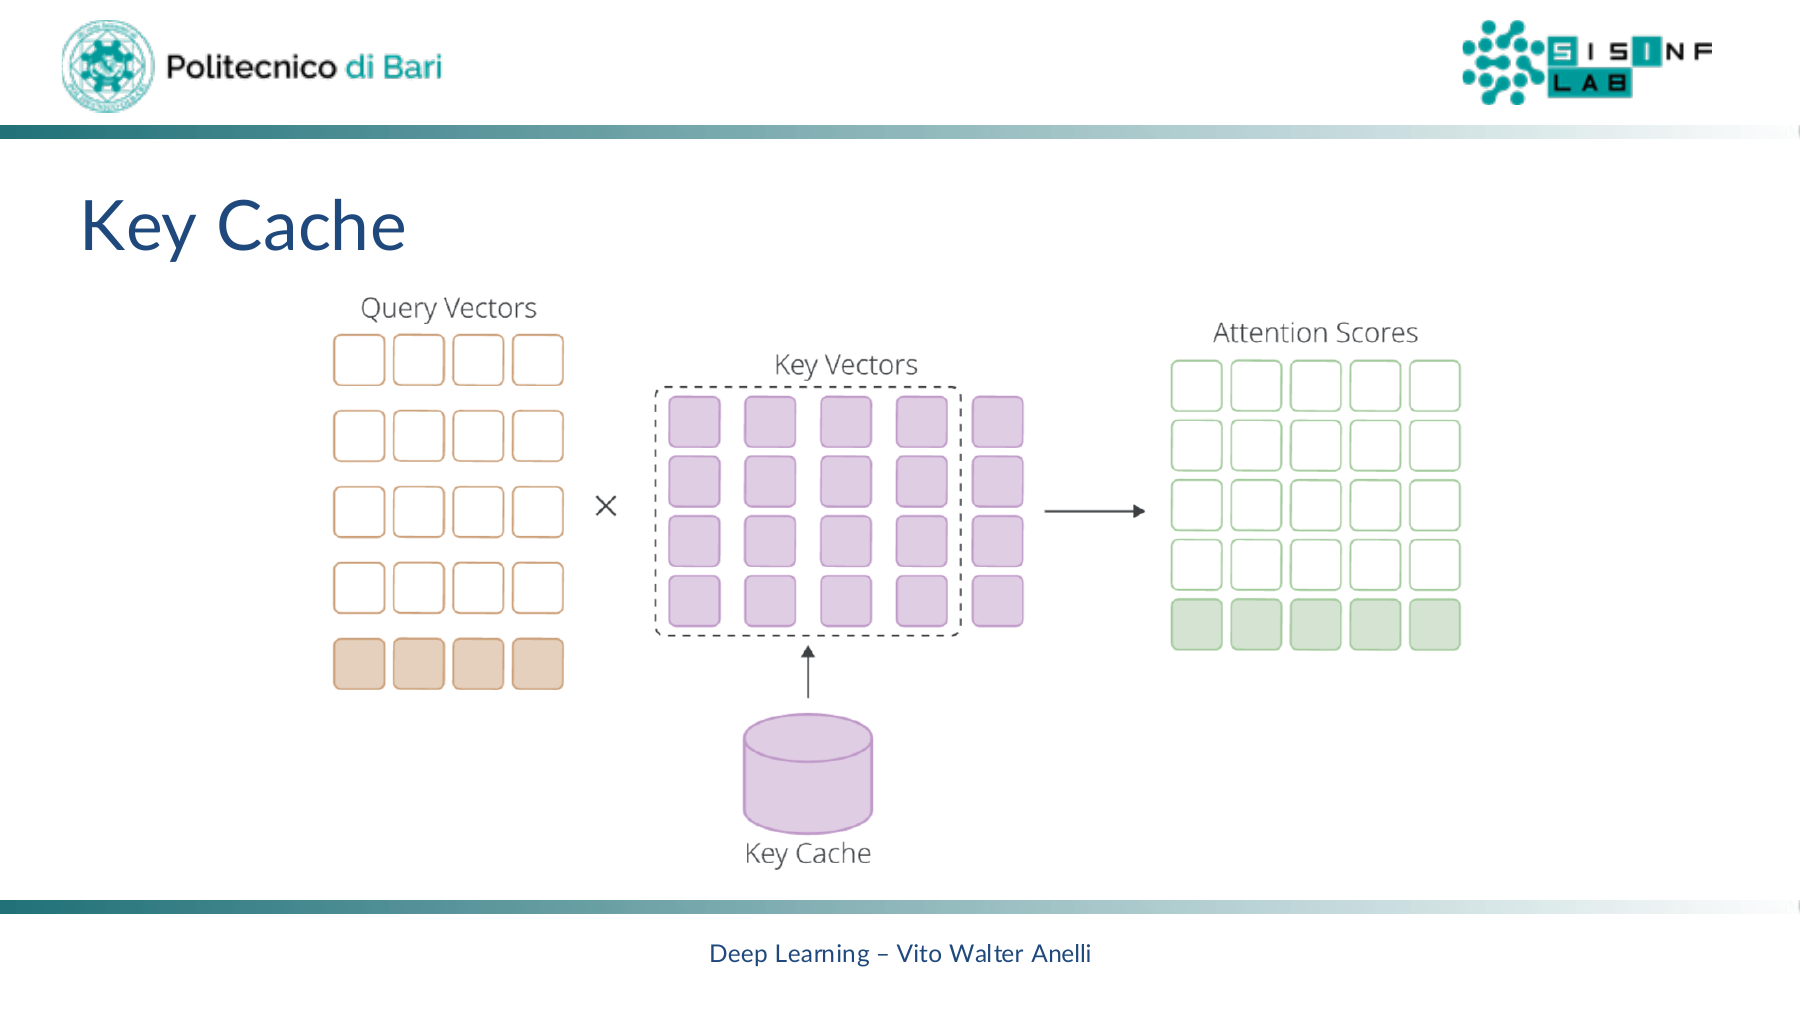
\includegraphics[width=0.80\linewidth]{figures/cf17_key_cache.png}
  \caption{Meccanismo della Key Cache. I vettori chiave dei token precedenti
           sono recuperati dalla cache (cilindro) ed usati direttamente nel
           prodotto scalare con il query del token corrente (riga arancione).}
  \label{fig:key-cache}
\end{figure}

\begin{figure}[H]
  \centering
  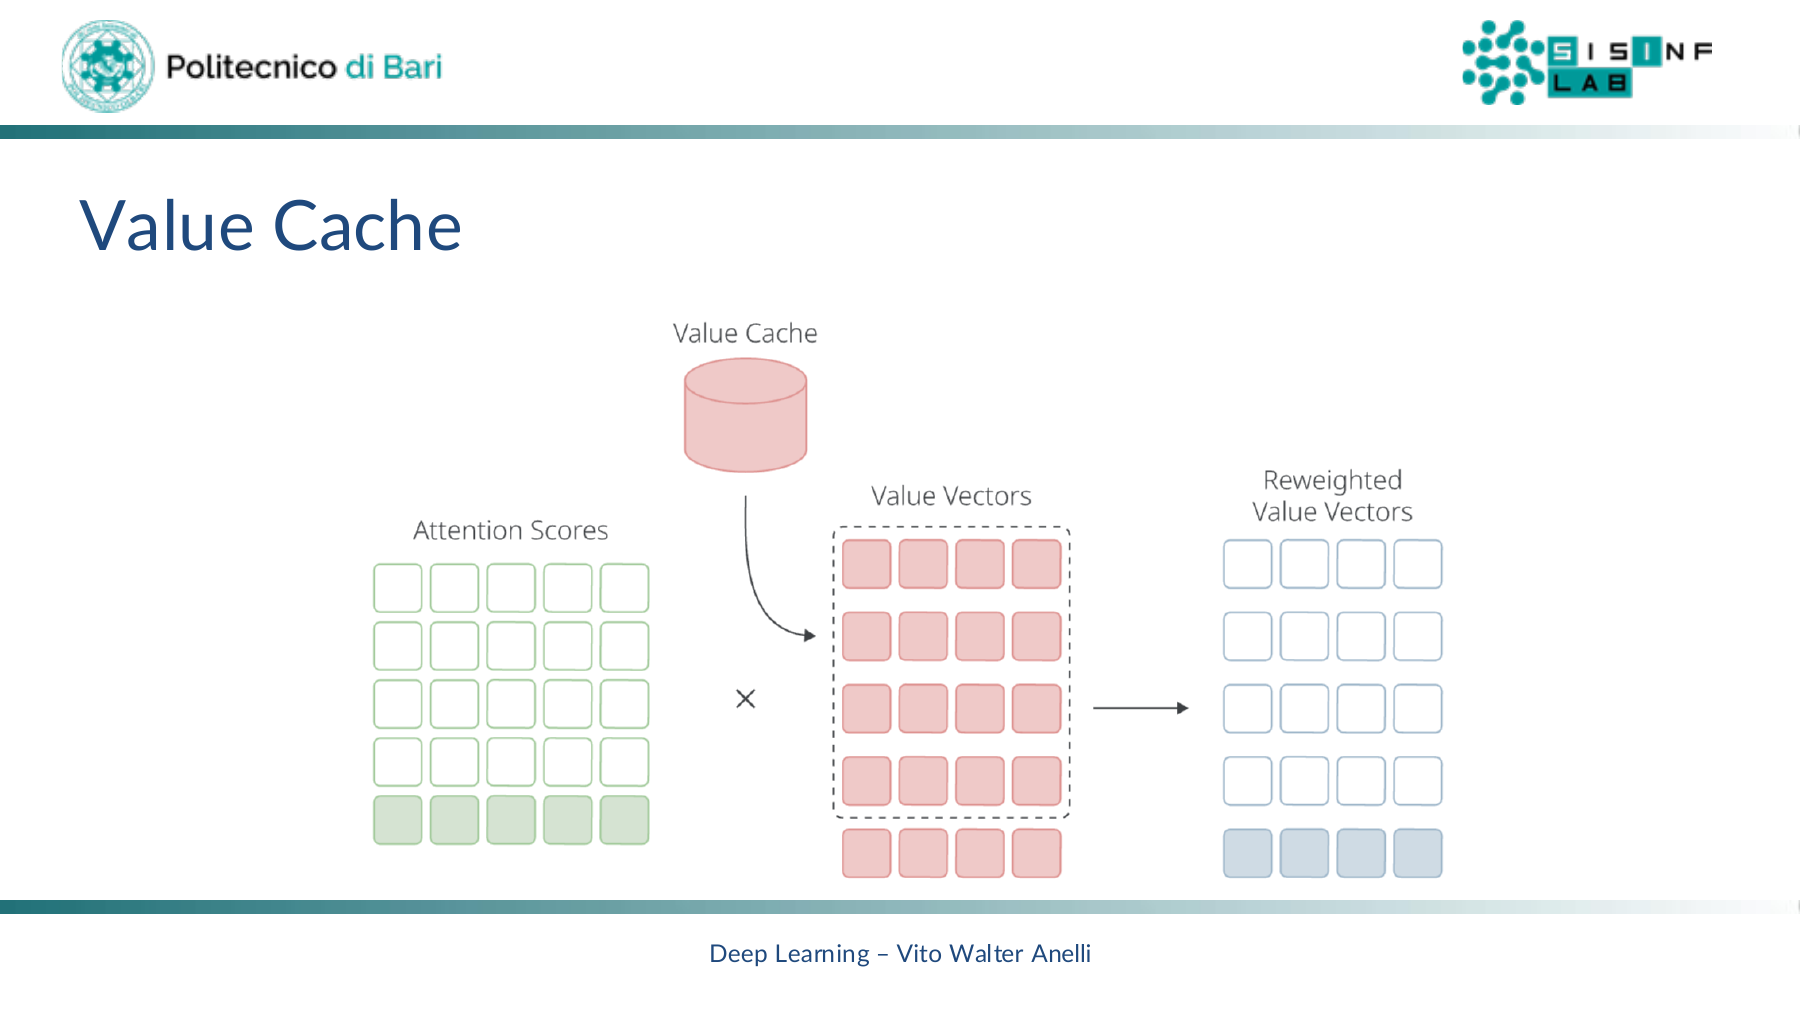
\includegraphics[width=0.80\linewidth]{figures/cf17_value_cache.png}
  \caption{Meccanismo della Value Cache. I vettori valore dei token precedenti
           sono recuperati dalla cache e usati nella somma pesata tramite
           i punteggi di attenzione del token corrente.}
  \label{fig:value-cache}
\end{figure}

\subsection{Dimensione della KV Cache}
\label{subsec:kv-cache-size}

La dimensione in memoria della KV Cache si determina considerando i seguenti
iper-parametri:

\begin{itemize}
  \item $l$: numero di layer del Transformer,
  \item $b$: batch size,
  \item $n$: numero di attention head,
  \item $h$: dimensione di ciascun head ($d_h$),
  \item $s$: lunghezza della sequenza.
\end{itemize}

Il tensore KV Cache per un singolo layer ha forma $(b,\, n,\, s,\, h)$.
Considerando sia le Key che i Value (fattore $\times 2$) e la
rappresentazione in mezza precisione FP16 ($2$ byte per elemento), la
dimensione totale in byte è:
\begin{equation}
  \text{KV Cache size} = l \times b \times n \times h \times s \times 2 \times 2
  \quad \text{[byte]}.
  \label{eq:kv-cache-size}
\end{equation}
A titolo d'esempio, per GPT-3 (175B parametri) con $b=1$ e $s=1024$, la KV
Cache occupa circa $4.5$ GB, una quantità non trascurabile rispetto alla VRAM
disponibile.

\begin{table}[H]
  \centering
  \caption{Dimensione della KV Cache (MHA standard) per le varianti di GPT-3
           con $b=1$, $s=1024$.}
  \label{tab:kv-cache-size-mha}
  \small
  \begin{tabular}{lrr}
    \toprule
    \textbf{Modello} & \textbf{Parametri} & \textbf{KV Cache} \\
    \midrule
    GPT-3 Small  & 125M  & 36 MB  \\
    GPT-3 Medium & 350M  & 96 MB  \\
    GPT-3 Large  & 760M  & 144 MB \\
    GPT-3 XL     & 1.3B  & 288 MB \\
    GPT-3 2.7B   & 2.7B  & 320 MB \\
    GPT-3 6.7B   & 6.7B  & 512 MB \\
    GPT-3 13B    & 13B   & 800 MB \\
    GPT-3        & 175B  & 4.5 GB \\
    \bottomrule
  \end{tabular}
\end{table}

%------------------------------------------------------------
\section{Multi-Query Attention}
\label{sec:mqa}

\subsection{Motivazione}
\label{subsec:mqa-motivation}

Nella MHA standard ogni head $i$ dispone di proiezioni Key e Value
\emph{indipendenti}: $W_K^{(i)}$ e $W_V^{(i)}$. La KV Cache deve quindi
memorizzare $n$ coppie $(K_i, V_i)$, il che scala linearmente con il numero
di head. La \textbf{Multi-Query Attention} (MQA) \citep{shazeer2019fast},
adottata in modelli come PaLM (Google) e Falcon, riduce questo costo
mantenendo un unico set di proiezioni Key e Value condiviso tra tutti
gli head delle query.

\subsection{Architettura}
\label{subsec:mqa-architecture}

Nella MQA si hanno $n$ proiezioni di query distinte, ma \textbf{una sola}
proiezione di Key e una sola di Value:
\begin{align}
  Q_i &= X W_Q^{(i)}, \quad i = 1,\ldots,n, \\
  K   &= X W_K, \\
  V   &= X W_V,
\end{align}
dove $W_K, W_V \in \mathbb{R}^{d_{\text{model}} \times d_h}$ sono le
proiezioni condivise. Il calcolo dell'attenzione per il head $i$ diventa:
\begin{equation}
  \text{head}_i = \text{Softmax}\!\left(\frac{Q_i K^\top}{\sqrt{d_h}}\right) V.
\end{equation}
Ogni head utilizza la stessa sequenza di chiavi e valori, ma con query
differenti, consentendo specializzazioni diverse nelle rappresentazioni
di output.

\begin{figure}[H]
  \centering
  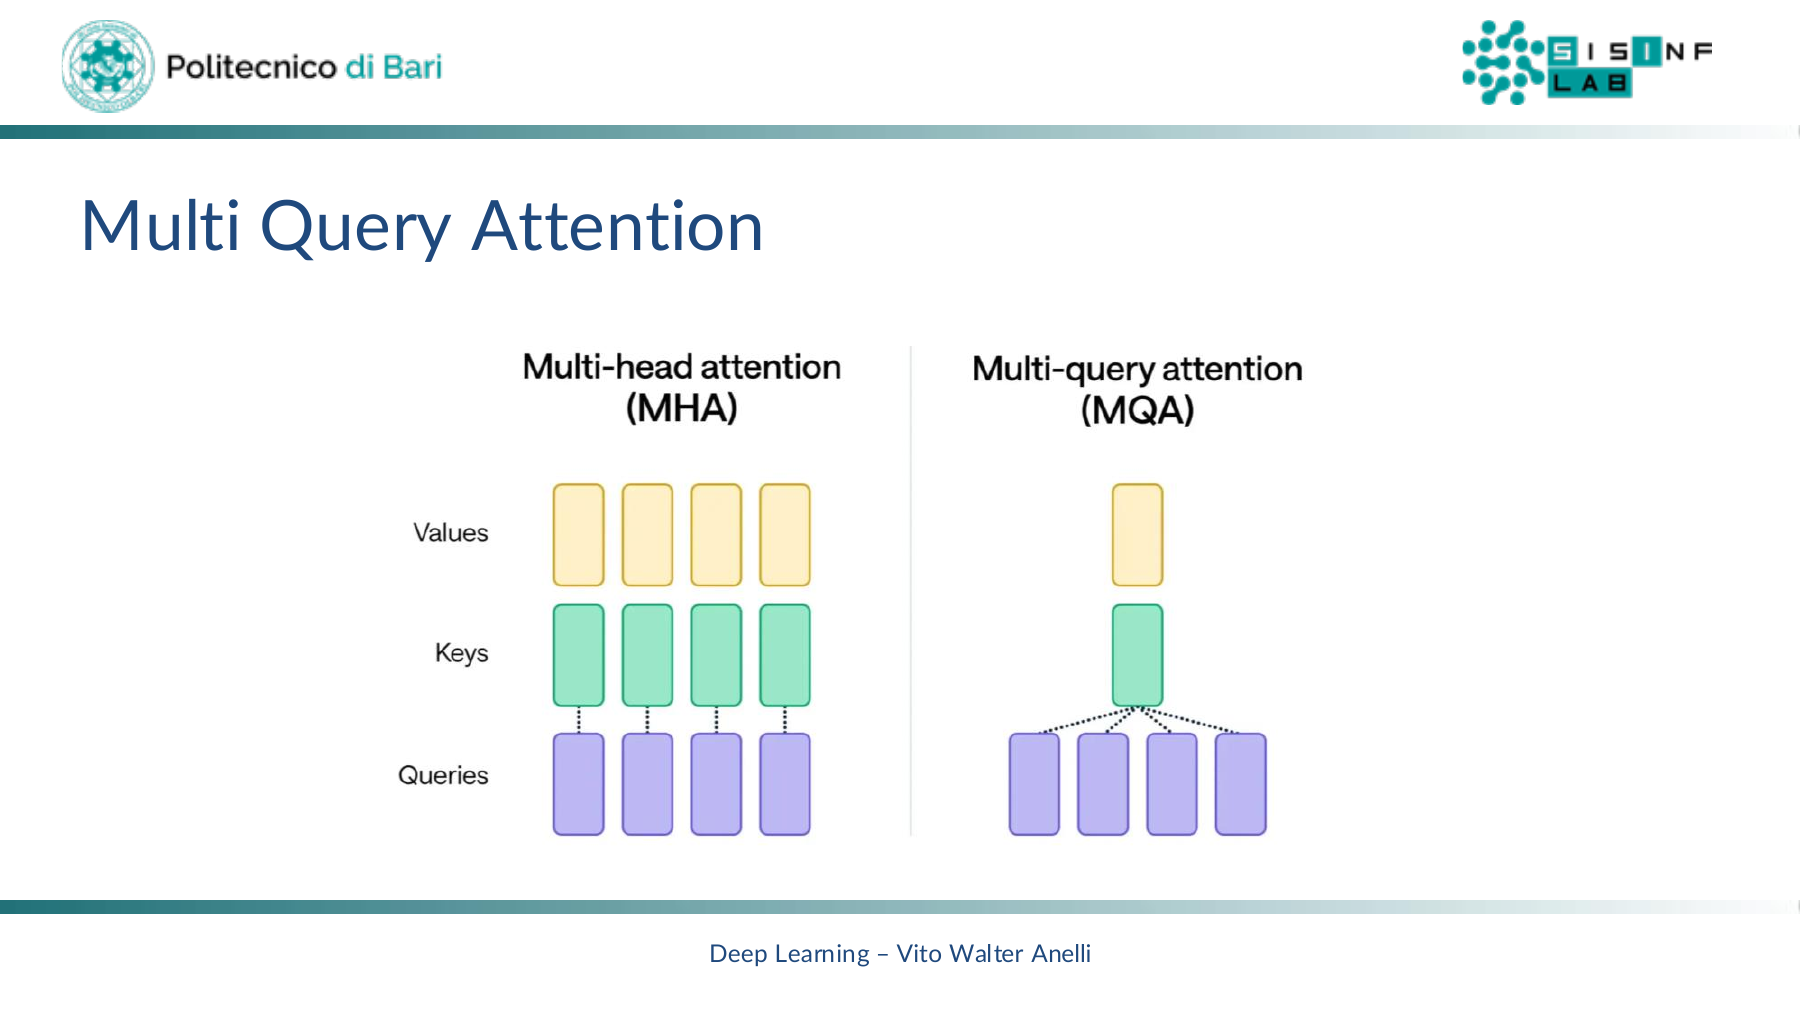
\includegraphics[width=0.72\linewidth]{figures/cf17_mha_vs_mqa.png}
  \caption{Confronto tra Multi-Head Attention (MHA) e Multi-Query Attention
           (MQA). In MHA ogni head possiede Key, Value e Query indipendenti.
           In MQA tutti gli head condividono un unico set di Key e Value,
           mentre le Query rimangono distinte.}
  \label{fig:mha-vs-mqa}
\end{figure}

\subsection{Dimensione della KV Cache con MQA}
\label{subsec:mqa-kv-cache}

Poiché Key e Value sono condivisi tra tutti gli $n$ head, la KV Cache
si riduce di un fattore $n$. La dimensione della cache con MQA è:
\begin{equation}
  \text{KV Cache size (MQA)} = l \times b \times s \times h \times 2 \times 2
  \quad \text{[byte]},
  \label{eq:kv-cache-size-mqa}
\end{equation}
che corrisponde esattamente all'equazione~\eqref{eq:kv-cache-size} senza
il fattore $n$. Il risparmio è quindi pari a $n$ volte rispetto alla MHA.

\begin{table}[H]
  \centering
  \caption{Confronto della dimensione della KV Cache tra MHA e MQA per le
           varianti di GPT-3, con $b=1$, $s=1024$.}
  \label{tab:kv-cache-mha-vs-mqa}
  \small
  \begin{tabular}{lrrr}
    \toprule
    \textbf{Modello} & \textbf{Parametri} & \textbf{KV Cache (MHA)} & \textbf{KV Cache (MQA)} \\
    \midrule
    GPT-3 Small  & 125M  & 36 MB   & 3 MB   \\
    GPT-3 Medium & 350M  & 96 MB   & 6 MB   \\
    GPT-3 Large  & 760M  & 144 MB  & 9 MB   \\
    GPT-3 XL     & 1.3B  & 288 MB  & 12 MB  \\
    GPT-3 2.7B   & 2.7B  & 320 MB  & 10 MB  \\
    GPT-3 6.7B   & 6.7B  & 512 MB  & 16 MB  \\
    GPT-3 13B    & 13B   & 800 MB  & 20 MB  \\
    GPT-3        & 175B  & 4.5 GB  & 48 MB  \\
    \bottomrule
  \end{tabular}
\end{table}

\subsection{Impatto sulle Prestazioni}
\label{subsec:mqa-performance}

La MQA introduce un leggero degrado qualitativo rispetto alla MHA, poiché
riduce la capacità espressiva dei Key e Value. Tuttavia, le valutazioni
empiriche su T5-XXL (Rouge score su CNN, arXiv, PubMed, MultiNews) e LLaMA~2
(zero-shot accuracy su BoolQ, PIQA, Hella-Swag, ARC-Easy) mostrano che il
degrado è contenuto, dell'ordine di 1--2 punti percentuali, a fronte di
un risparmio di memoria di un ordine di grandezza \citep{shazeer2019fast}.

%------------------------------------------------------------
\section{Grouped-Query Attention}
\label{sec:gqa}

\subsection{Motivazione e Architettura}
\label{subsec:gqa-architecture}

La \textbf{Grouped-Query Attention} (GQA) \citep{ainslie2023gqa}, adottata
in LLaMA~2, LLaMA~3 e Mistral 7B, rappresenta un compromesso continuo tra
MHA e MQA. Gli $n$ head di query vengono suddivisi in $G$ gruppi ($G$
divisore di $n$), dove ogni gruppo condivide un unico set di Key e Value.
Con $G = 1$ si recupera la MQA; con $G = n$ si recupera la MHA.

Definendo $n_g = n / G$ il numero di query head per gruppo, le proiezioni sono:
\begin{align}
  Q_i     &= X W_Q^{(i)}, \quad i = 1,\ldots,n, \\
  K_{[g]} &= X W_K^{(g)}, \quad g = 1,\ldots,G, \\
  V_{[g]} &= X W_V^{(g)}, \quad g = 1,\ldots,G.
\end{align}
Il head $i$, appartenente al gruppo $g(i) = \lceil i\,n/G \rceil$, calcola:
\begin{equation}
  \text{head}_i = \text{Softmax}\!\left(
    \frac{Q_i K_{[g(i)]}^\top}{\sqrt{d_h}}
  \right) V_{[g(i)]}.
\end{equation}

\begin{figure}[H]
  \centering
  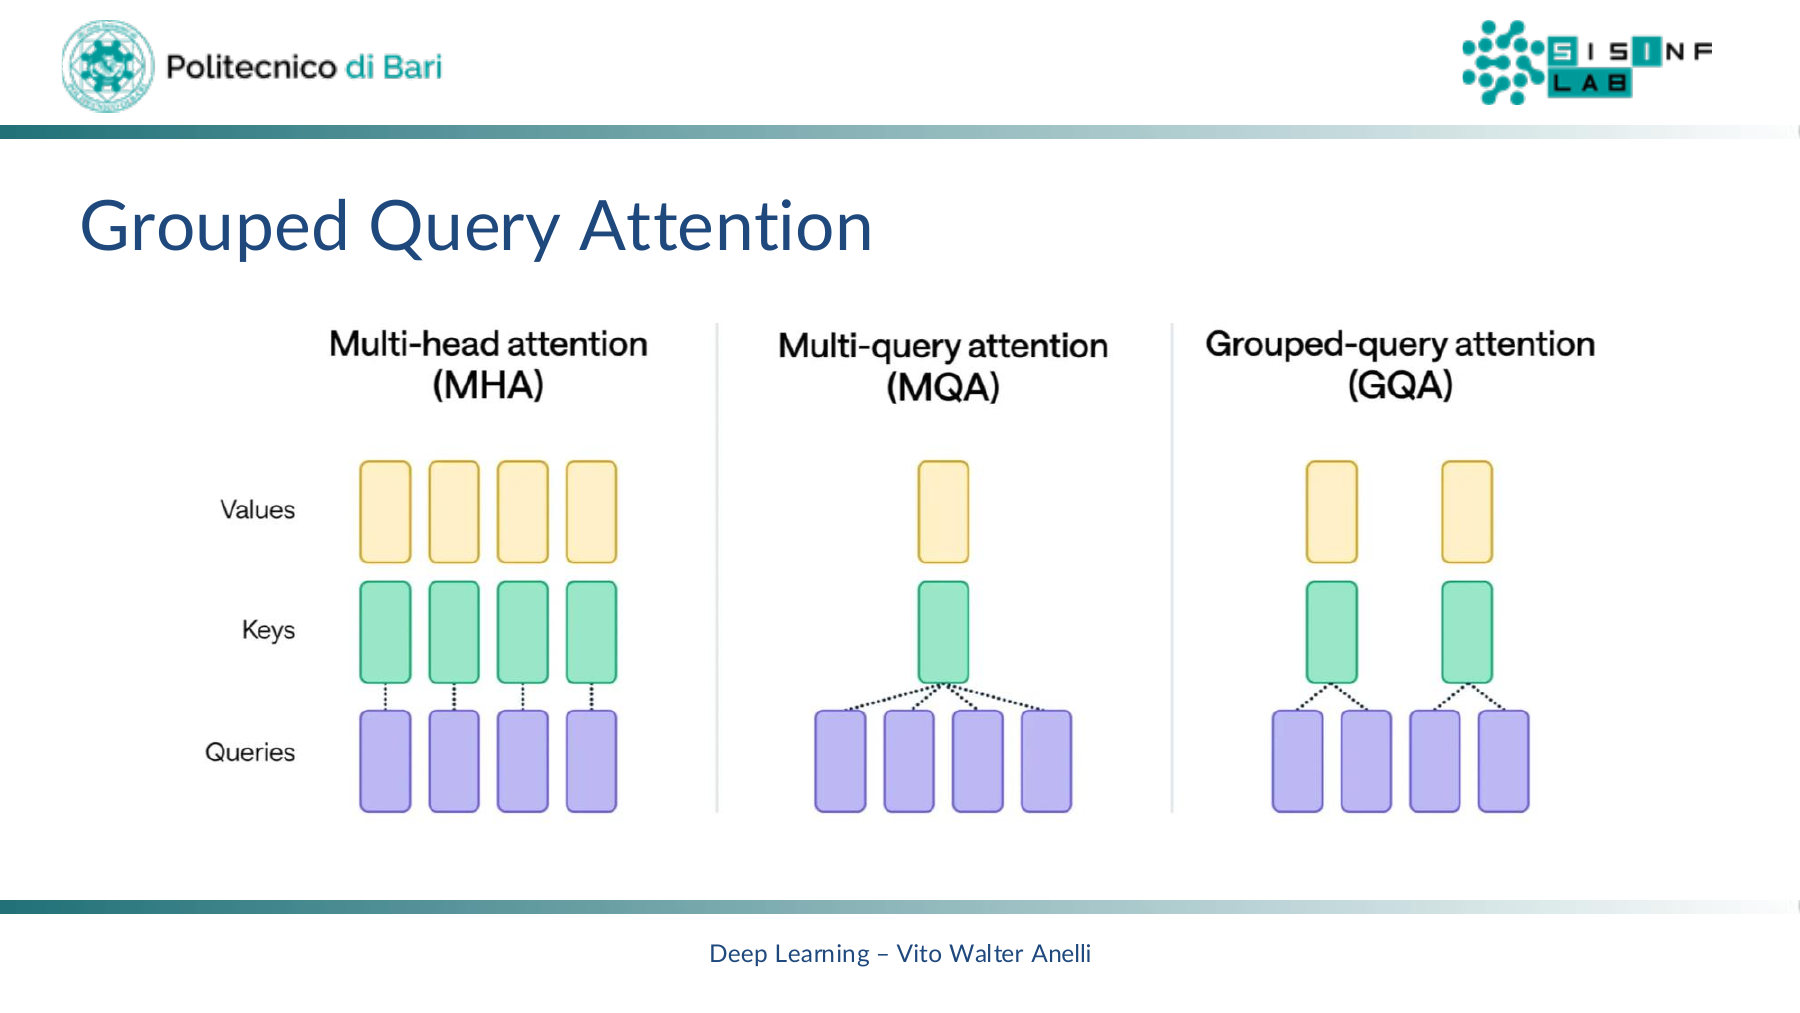
\includegraphics[width=0.85\linewidth]{figures/cf17_mha_mqa_gqa.png}
  \caption{Confronto tra MHA, MQA e GQA. In GQA gli $n$ head di query sono
           divisi in $G$ gruppi, ognuno con le proprie Key e Value condivise
           tra i membri del gruppo. Con $G=n$ si ottiene MHA, con $G=1$
           si ottiene MQA.}
  \label{fig:gqa}
\end{figure}

\subsection{Dimensione della KV Cache con GQA}
\label{subsec:gqa-kv-cache}

La KV Cache con GQA scala con il numero di gruppi $G$:
\begin{equation}
  \text{KV Cache size (GQA)} = l \times b \times G \times h \times s \times 2 \times 2
  \quad \text{[byte]}.
  \label{eq:kv-cache-size-gqa}
\end{equation}
Il risparmio rispetto alla MHA è pari a $n/G$: con $G=8$ e $n=32$ si ottiene
un fattore $4\times$ di riduzione, con un degrado qualitativo inferiore
rispetto alla MQA.

\subsection{Impatto sulle Prestazioni}
\label{subsec:gqa-performance}

La GQA con $G=8$ su T5-XXL raggiunge prestazioni molto vicine alla MHA
(entro 0.5 punti Rouge), superando la MQA in tutti i benchmark considerati.
Questo rende la GQA la scelta preferita nei modelli di grandi dimensioni
moderni, in quanto offre un ottimo compromesso tra efficienza della memoria
e capacità del modello \citep{ainslie2023gqa}.

%------------------------------------------------------------
\section{Rotary Positional Embeddings (RoPE)}
\label{sec:rope}

\subsection{Limiti degli Embedding Posizionali Assoluti}
\label{subsec:absolute-pe-limits}

Gli embedding posizionali assoluti (come quelli originali del Transformer
\citep{vaswani2017attention}) assegnano a ciascuna posizione $m$ un vettore
fisso $\mathbf{p}_m$, sommato all'embedding del token prima dell'attenzione.
Questa formulazione presenta due limiti fondamentali:

\begin{itemize}
  \item \textbf{Lunghezza massima fissa}: il modello non può rappresentare
        posizioni oltre la lunghezza massima vista durante il training.
  \item \textbf{Indipendenza posizionale}: ogni embedding è indipendente
        dagli altri. Il modello tratta la differenza tra le posizioni $1$ e $2$
        allo stesso modo della differenza tra le posizioni $2$ e $500$,
        ostacolando la comprensione della struttura relativa della sequenza.
\end{itemize}

\subsection{Embedding Posizionali Relativi}
\label{subsec:relative-pe}

Gli embedding posizionali relativi (ad esempio in T5 \citep{raffel2020t5})
modellano la \emph{distanza} tra coppie di token anziché la loro posizione
assoluta. In T5, un bias scalare $b(m-n)$ viene aggiunto alla matrice di
attenzione $Q K^\top$ tra il token in posizione $m$ e quello in posizione $n$:
\begin{equation}
  A_{mn} \leftarrow \frac{\mathbf{q}_m \cdot \mathbf{k}_n}{\sqrt{d_h}} + b(m-n).
\end{equation}
Sebbene concettualmente più ricchi, gli embedding relativi presentano
problemi pratici:
\begin{itemize}
  \item Maggiore costo computazionale, specialmente per sequenze lunghe.
  \item \textbf{Incompatibilità con la KV Cache}: aggiungere un nuovo token
        modifica l'embedding relativo di tutti i token precedenti,
        invalidando la cache.
\end{itemize}
Per questi motivi, gli embedding relativi non hanno trovato ampia adozione
nei grandi modelli linguistici.

\subsection{Matrice di Rotazione}
\label{subsec:rotation-matrix}

Alla base di RoPE vi è la \textbf{matrice di rotazione 2D}, che ruota un
vettore di un angolo $\theta$ preservandone la norma:
\begin{equation}
  R(\theta) = \begin{pmatrix} \cos\theta & -\sin\theta \\ \sin\theta & \cos\theta \end{pmatrix},
  \qquad
  R(\theta)\,\mathbf{x} = \begin{pmatrix} \cos\theta\, x_1 - \sin\theta\, x_2 \\
                                            \sin\theta\, x_1 + \cos\theta\, x_2 \end{pmatrix}.
  \label{eq:rotation-matrix}
\end{equation}
La moltiplicazione per $R(\theta)$ cambia la direzione del vettore senza
alterarne la lunghezza. Questa proprietà è fondamentale per costruire
embedding posizionali che si comportino bene nel prodotto scalare.

\subsection{Formulazione di RoPE}
\label{subsec:rope-formulation}

I \textbf{Rotary Positional Embeddings} (RoPE) \citep{su2024rope}, adottati in
RoFormer, LLaMA~2/3, Gemma, PaLM, GPT-NeoX, Falcon e DeepSeek, incorporano
l'informazione posizionale \emph{all'interno} del calcolo del prodotto
scalare tra query e key, anziché aggiungerla agli embedding di input.

Per un vettore di query o key a $d_h$ dimensioni nella posizione $m$, RoPE
applica una rotazione dipendente dalla posizione. Nel caso 2D, la query
$\mathbf{q} = W_Q \mathbf{x}$ viene trasformata come:
\begin{equation}
  \text{RoPE}(\mathbf{q}, m) = R(m\theta)\, W_Q\, \mathbf{x}
  = \begin{pmatrix} \cos m\theta & -\sin m\theta \\
                    \sin m\theta & \phantom{-}\cos m\theta \end{pmatrix}
    W_Q \begin{pmatrix} x_1 \\ x_2 \end{pmatrix}.
  \label{eq:rope-query}
\end{equation}
Analogamente, la key in posizione $n$ viene trasformata con $R(n\theta)$.

Le rotazioni godono della seguente proprietà algebrica:

\begin{theorem}[Prodotto tra rotazioni]
Per qualsiasi angolo $\alpha, \beta$:
\begin{equation}
  R(\alpha)^\top R(\beta) = R(\beta - \alpha).
  \label{eq:rotation-product}
\end{equation}
\end{theorem}

Applicando questo risultato al calcolo del punteggio di attenzione tra i
token in posizione $m$ e $n$:
\begin{align}
  \text{score}(m, n)
    &= \mathbf{q}_m^\top \mathbf{k}_n \notag \\
    &= \bigl(R(m\theta)\,\mathbf{q}\bigr)^\top \bigl(R(n\theta)\,\mathbf{k}\bigr) \notag \\
    &= \mathbf{q}^\top R(m\theta)^\top R(n\theta)\,\mathbf{k} \notag \\
    &= \mathbf{q}^\top R\bigl((n-m)\theta\bigr)\,\mathbf{k}.
  \label{eq:rope-score}
\end{align}
Il punteggio di attenzione dipende quindi solo dalla \textbf{distanza
relativa} $n - m$ tra i due token, non dalle posizioni assolute. Questo
garantisce la proprietà degli embedding relativi, pur essendo applicato
localmente alle singole coppie (query, key).

\begin{figure}[H]
  \centering
  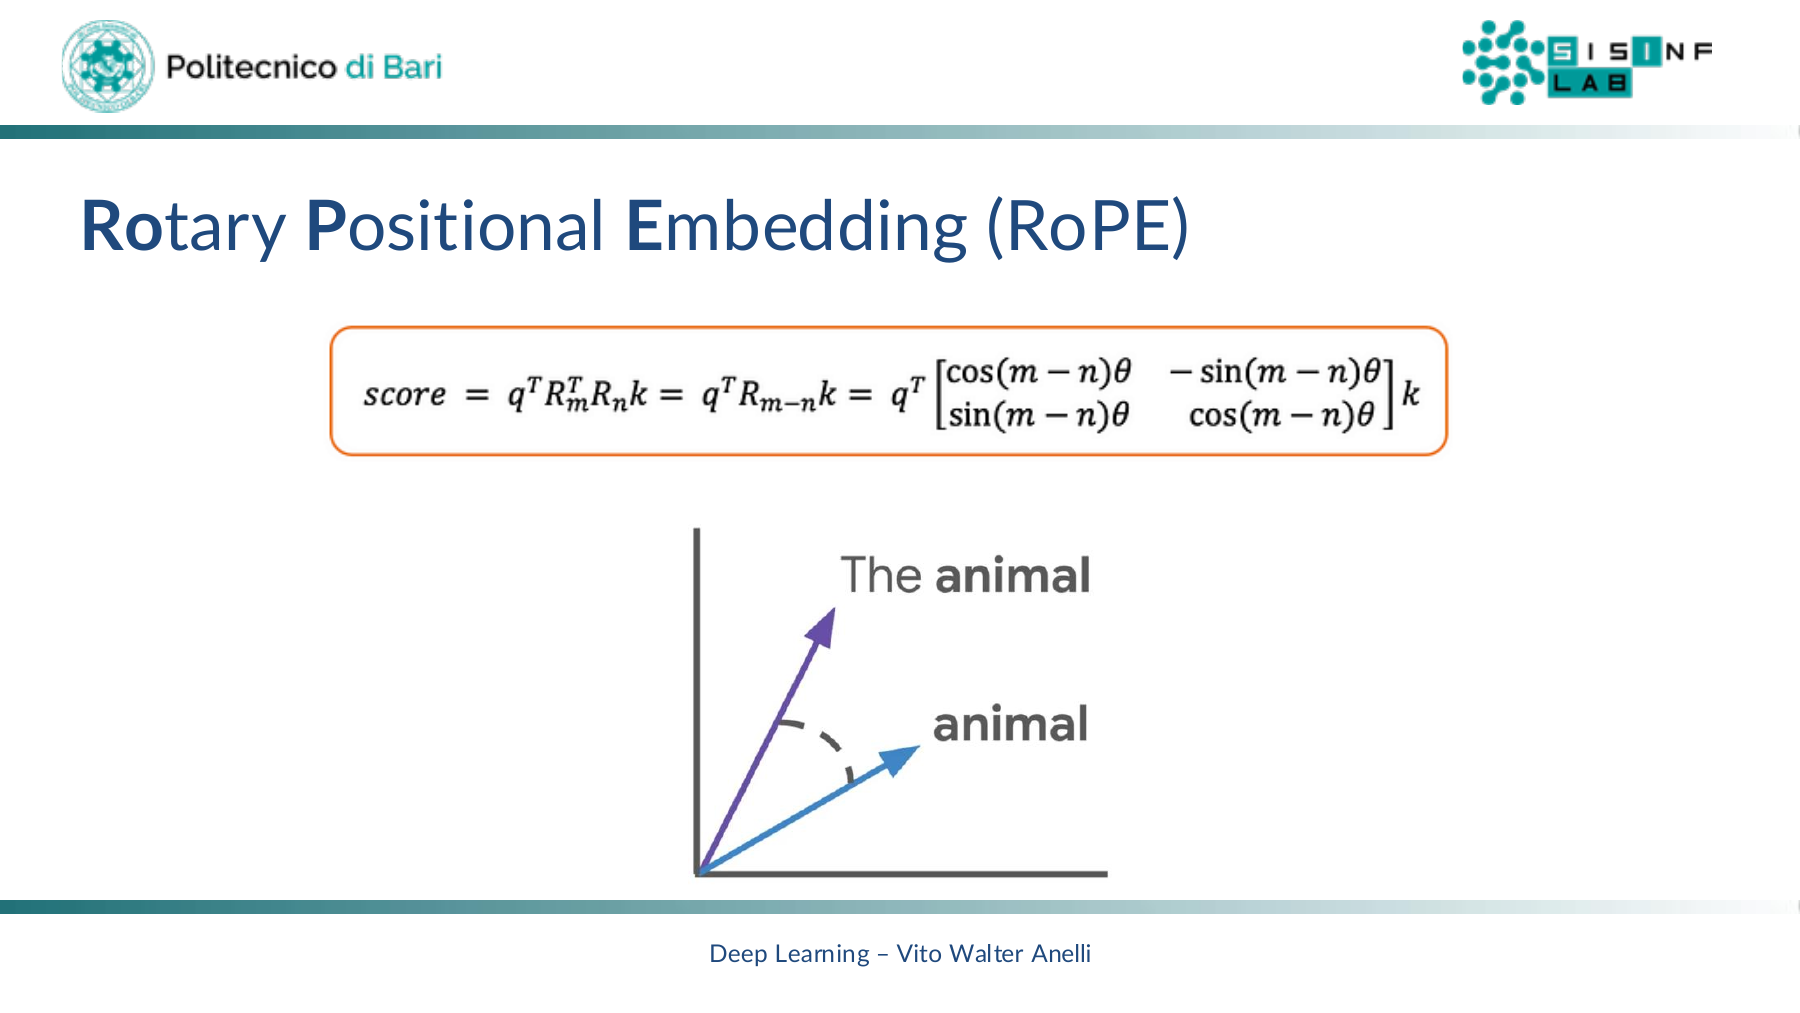
\includegraphics[width=0.62\linewidth]{figures/cf17_rope_score.png}
  \caption{Interpretazione geometrica di RoPE. La parola \emph{animal}
           appare in due posizioni diverse nella sequenza; RoPE la rappresenta
           come due vettori ruotati di angoli diversi. Il prodotto scalare
           tra la query e la key cattura la distanza relativa tra le due
           occorrenze.}
  \label{fig:rope-score}
\end{figure}

\subsection{Estensione a dimensioni superiori}
\label{subsec:rope-higher-dim}

In pratica $d_h > 2$. RoPE estende la formulazione 2D suddividendo il
vettore di query (o key) in $d_h/2$ coppie di dimensioni, applicando
a ciascuna coppia $(x_{2i-1}, x_{2i})$ una rotazione di angolo $m\theta_i$,
con frequenze geometricamente spaziate:
\begin{equation}
  \theta_i = \theta_{\text{base}}^{-2(i-1)/d_h},
  \qquad \theta_{\text{base}} = 10000 \text{ (default)}.
  \label{eq:rope-freq}
\end{equation}
Le basse frequenze catturano strutture di lungo raggio, le alte frequenze
strutture locali, in modo analogo agli embedding sinusoidali originali di
\citet{vaswani2017attention} ma con la proprietà aggiuntiva di essere
compatibili con la KV Cache.

\paragraph{Compatibilità con la KV Cache.}
Poiché RoPE agisce localmente sui vettori query e key (anziché sugli
embedding di input), i vettori chiave già memorizzati nella cache rimangono
validi: è sufficiente applicare la rotazione $R(m\theta)$ alla key del
nuovo token prima di inserirla in cache.

%------------------------------------------------------------
\section{Multi-Head Latent Attention}
\label{sec:mla}

\subsection{Motivazione}
\label{subsec:mla-motivation}

La \textbf{Multi-Head Latent Attention} (MLA) \citep{deepseekv2_2024},
introdotta in DeepSeek V2/V3/R1, propone un'alternativa radicalmente diversa
a MQA e GQA per ridurre la KV Cache. Invece di ridurre il numero di head
per Key e Value, MLA \textbf{comprime} l'intera rappresentazione KV in un
vettore latente di bassa dimensione, che viene poi espanso quando serve.

\subsection{Compressione della KV Cache}
\label{subsec:mla-compression}

Dato il vettore di input $\mathbf{h}_t \in \mathbb{R}^{d}$ al passo $t$
(dove $d = n_h \cdot d_h$ è la dimensione del modello), la proiezione
\emph{down-projection} comprime $\mathbf{h}_t$ in un vettore latente di
dimensione $d_c \ll d$:
\begin{equation}
  \mathbf{c}_t^{KV} = W^{DKV} \mathbf{h}_t,
  \qquad W^{DKV} \in \mathbb{R}^{d_c \times d}.
  \label{eq:mla-compress}
\end{equation}
Quando è necessario calcolare l'attenzione, Key e Value vengono recuperati
tramite le proiezioni \emph{up-projection}:
\begin{equation}
  \mathbf{k}_t^C = W^{UK} \mathbf{c}_t^{KV},
  \qquad
  \mathbf{v}_t^C = W^{UV} \mathbf{c}_t^{KV},
  \label{eq:mla-up-kv}
\end{equation}
dove $W^{UK}, W^{UV} \in \mathbb{R}^{(n_h d_h) \times d_c}$ sono le
matrici di espansione. Nella cache viene memorizzato \textbf{solo}
$\mathbf{c}_t^{KV}$, non le Key e Value espanse.

Analogamente, anche le query vengono compresse e poi espanse:
\begin{equation}
  \mathbf{c}_t^Q = W^{DQ} \mathbf{h}_t, \qquad
  \mathbf{q}_t^C = W^{UQ} \mathbf{c}_t^Q.
  \label{eq:mla-query}
\end{equation}

\begin{figure}[H]
  \centering
  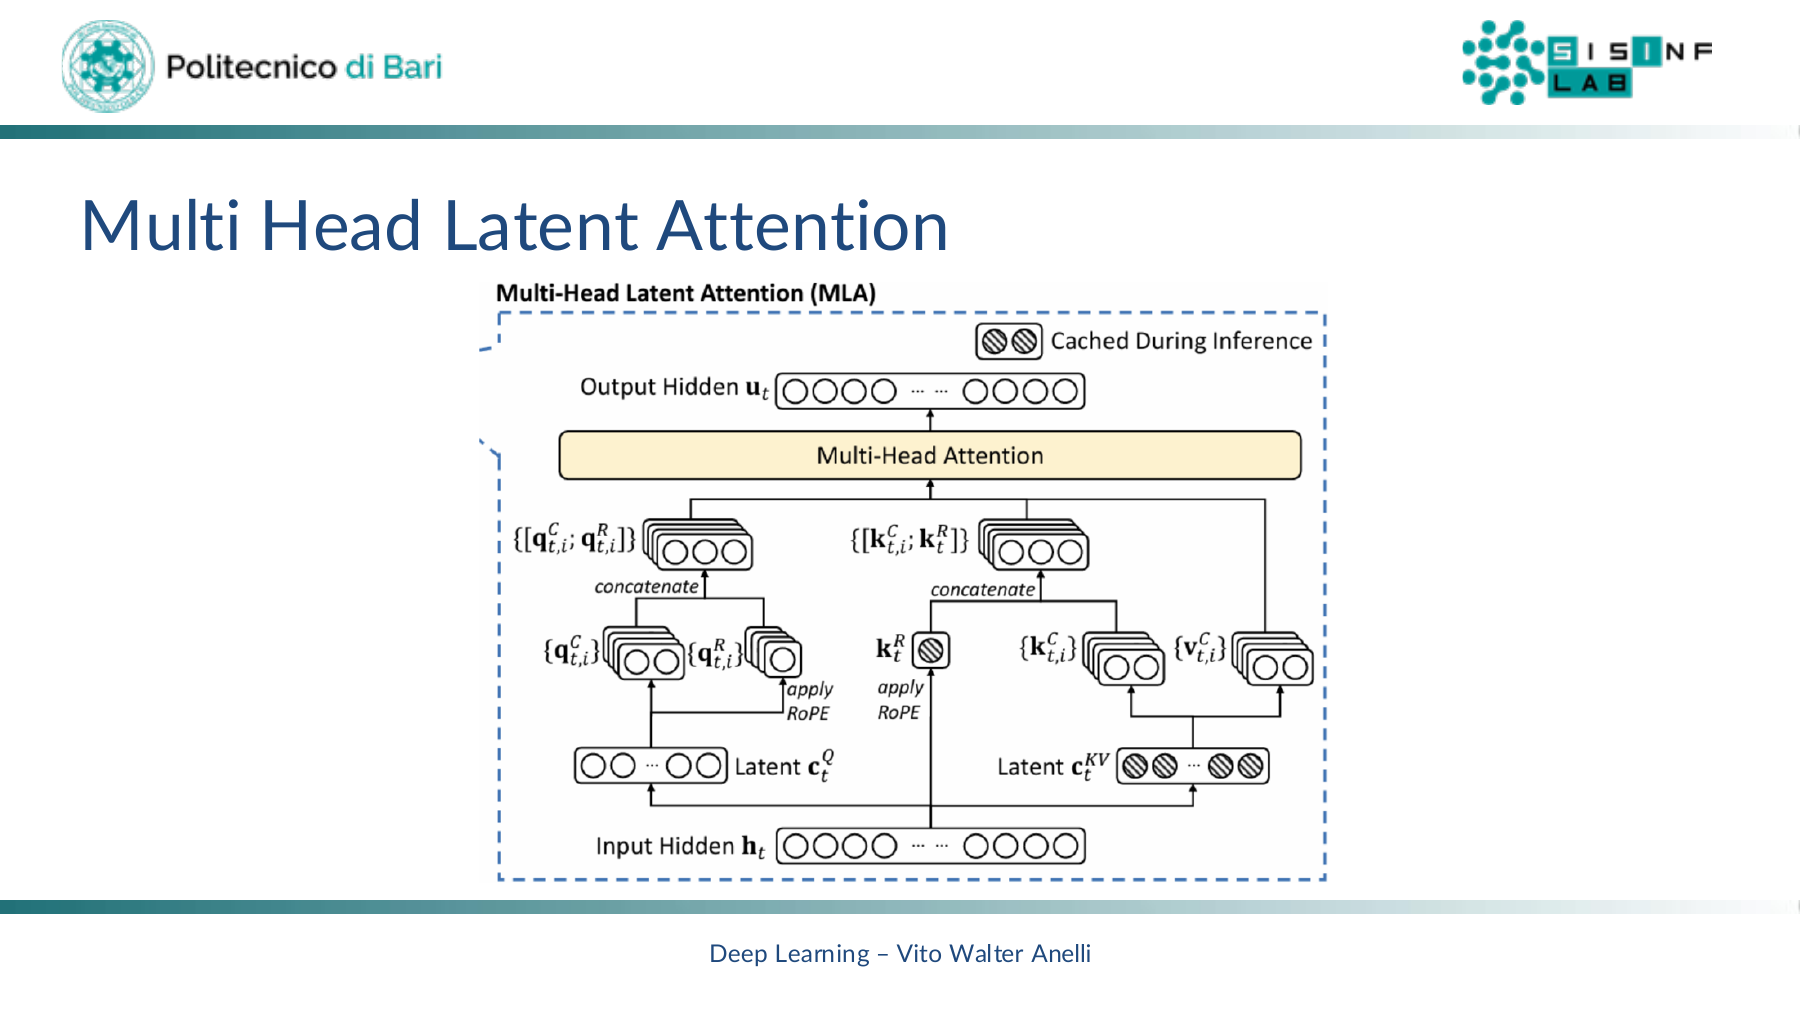
\includegraphics[width=0.85\linewidth]{figures/cf17_mla_architecture.png}
  \caption{Schema completo della Multi-Head Latent Attention (MLA). Il
           vettore di input $\mathbf{h}_t$ viene proiettato in due vettori
           latenti $\mathbf{c}_t^Q$ e $\mathbf{c}_t^{KV}$ (dimensione
           ridotta). Solo $\mathbf{c}_t^{KV}$ viene memorizzato in cache.
           Le query, le key e i value vengono ricostruiti tramite
           up-projection prima del calcolo dell'attenzione. Le chiavi RoPE
           sono calcolate separatamente e concatenate (decoupled RoPE).}
  \label{fig:mla-architecture}
\end{figure}

\subsection{Assorbimento delle matrici di proiezione}
\label{subsec:mla-absorption}

Un'osservazione chiave è che, nel calcolo del punteggio di attenzione tra
$\mathbf{q}_t^C$ e $\mathbf{k}_t^C$, le matrici $W^{UQ}$ e $W^{UK}$
compaiono sempre insieme:
\begin{equation}
  \mathbf{q}_t^{C\top} \mathbf{k}_t^C
  = \mathbf{c}_t^{Q\top}\bigl(W^{UQ}\bigr)^\top W^{UK} \mathbf{c}_t^{KV}.
\end{equation}
Il prodotto $\bigl(W^{UQ}\bigr)^\top W^{UK}$ può essere precalcolato e
``assorbito'' in $W^{UQ}$, riducendo ulteriormente il numero di parametri
da mantenere in memoria durante l'inferenza.

\subsection{RoPE Disaccoppiata}
\label{subsec:decoupled-rope}

L'applicazione diretta di RoPE alle key compresse è \textbf{incompatibile}
con la strategia di assorbimento: la matrice di rotazione $R(m\theta)$
dipende dalla posizione e non può essere assorbita in $W^{UQ}$ (verrebbe
inserita tra i due fattori della moltiplicazione, impedendo la fusione).

La soluzione proposta in \citet{deepseekv2_2024} è il \textbf{RoPE
disaccoppiato}: si introducono vettori di query e key ausiliari
$\mathbf{q}_t^R$ e $\mathbf{k}_t^R$, dedicati esclusivamente alla
codifica posizionale tramite RoPE:
\begin{align}
  \mathbf{q}_t^R &= \text{RoPE}(W^{QR} \mathbf{c}_t^Q, \; t), \\
  \mathbf{k}_t^R &= \text{RoPE}(W^{KR} \mathbf{h}_t, \; t).
\end{align}
Il key condiviso $\mathbf{k}_t^R$ è un singolo vettore per tutte le head
(come in MQA), e viene anch'esso memorizzato in cache. La query e la key
finali sono formate per concatenazione:
\begin{align}
  \mathbf{q}_{t,i} &= [\mathbf{q}_{t,i}^C;\, \mathbf{q}_{t,i}^R], \\
  \mathbf{k}_{t,i} &= [\mathbf{k}_{t,i}^C;\, \mathbf{k}_t^R].
\end{align}

\subsection{Calcolo Completo di MLA}
\label{subsec:mla-computation}

Il calcolo completo di MLA, comprensivo di RoPE disaccoppiata, è il seguente
(Equazioni 37--47 di \citet{deepseekv2_2024}):
\begin{align}
  \mathbf{c}_t^Q &= W^{DQ}\mathbf{h}_t, \tag{37} \\
  [\mathbf{q}_{t,1}^C;\ldots;\mathbf{q}_{t,n_h}^C]
    &= \mathbf{q}_t^C = W^{UQ}\mathbf{c}_t^Q, \tag{38} \\
  [\mathbf{q}_{t,1}^R;\ldots;\mathbf{q}_{t,n_h}^R]
    &= \mathbf{q}_t^R = \text{RoPE}(W^{QR}\mathbf{c}_t^Q), \tag{39} \\
  \mathbf{q}_{t,i} &= [\mathbf{q}_{t,i}^C;\,\mathbf{q}_{t,i}^R], \tag{40} \\[4pt]
  \mathbf{c}_t^{KV} &= W^{DKV}\mathbf{h}_t, \tag{41} \\
  [\mathbf{k}_{t,1}^C;\ldots;\mathbf{k}_{t,n_h}^C]
    &= \mathbf{k}_t^C = W^{UK}\mathbf{c}_t^{KV}, \tag{42} \\
  \mathbf{k}_t^R &= \text{RoPE}(W^{KR}\mathbf{h}_t), \tag{43} \\
  \mathbf{k}_{t,i} &= [\mathbf{k}_{t,i}^C;\,\mathbf{k}_t^R], \tag{44} \\
  [\mathbf{v}_{t,1}^C;\ldots;\mathbf{v}_{t,n_h}^C]
    &= \mathbf{v}_t^C = W^{UV}\mathbf{c}_t^{KV}, \tag{45} \\[4pt]
  \mathbf{o}_{t,i}
    &= \sum_{j=1}^{t} \text{Softmax}_j\!\left(
        \frac{\mathbf{q}_{t,i}^\top \mathbf{k}_{j,i}}{\sqrt{d_h + d_h^R}}
      \right) \mathbf{v}_{j,i}^C, \tag{46} \\
  \mathbf{u}_t &= W^O\,[\mathbf{o}_{t,1};\ldots;\mathbf{o}_{t,n_h}]. \tag{47}
\end{align}

\noindent In cache si memorizzano \textbf{solo} $\mathbf{c}_t^{KV}$ e
$\mathbf{k}_t^R$, ovvero un vettore di dimensione $d_c + d_h^R$ per token per
layer.

\subsection{Dimensione della KV Cache con MLA}
\label{subsec:mla-kv-size}

La tabella seguente confronta la dimensione della KV Cache per token per layer
e la capacità del modello tra i quattro meccanismi di attenzione discussi.

\begin{table}[H]
  \centering
  \caption{Confronto della KV Cache per token per layer e della capacità del
           modello tra le varianti di attention (da \citet{deepseekv2_2024}).
           $n_h$: numero di head; $d_h$: dimensione del head; $n_g$: numero
           di gruppi GQA; $d_c$: dimensione latente MLA; $d_h^R$: dimensione
           della componente RoPE.}
  \label{tab:attention-comparison}
  \small
  \begin{tabular}{lccc}
    \toprule
    \textbf{Meccanismo} & \textbf{KV Cache per token} & \textbf{Capacità} \\
    \midrule
    Multi-Head Attention (MHA)   & $2 n_h d_h l$              & Forte    \\
    Grouped-Query Attention (GQA) & $2 n_g d_h l$             & Moderata \\
    Multi-Query Attention (MQA)  & $2 d_h l$                  & Debole   \\
    \midrule
    MLA (DeepSeek)               & $(d_c + d_h^R)\,l \approx \tfrac{9}{2} d_h l$ & Più forte \\
    \bottomrule
  \end{tabular}
\end{table}

\noindent Nonostante la KV Cache di MLA sia paragonabile a quella di GQA con
un numero ridotto di gruppi, i benchmark su modelli Dense~7B e MoE mostrano
che MLA supera MHA sia in qualità (BBH, MMLU, C-Eval, CMMLU) sia in efficienza
di memoria, grazie alla ricchezza semantica del vettore latente compresso
\citep{deepseekv2_2024}.

%------------------------------------------------------------
\section{Riepilogo e Confronto}
\label{sec:attention-summary}

\begin{table}[H]
  \centering
  \caption{Riepilogo delle varianti di Multi-Head Attention. $n$: numero di
           head; $G$: numero di gruppi GQA; $d_c$: dimensione latente MLA.}
  \label{tab:attention-summary}
  \small
  \begin{tabular}{lcccc}
    \toprule
    \textbf{Meccanismo} & \textbf{Key/Value head} & \textbf{KV Cache} & \textbf{Qualità} & \textbf{Adottato in} \\
    \midrule
    MHA  & $n$ indipendenti  & $O(n)$     & Massima  & GPT, BERT \\
    MQA  & 1 condiviso       & $O(1)$     & Ridotta  & PaLM, Falcon \\
    GQA  & $G$ condivisi     & $O(G)$     & Alta     & LLaMA 2/3, Mistral \\
    MLA  & Vettore latente   & $O(d_c/d)$ & Massima+ & DeepSeek V2/V3/R1 \\
    \bottomrule
  \end{tabular}
\end{table}

\paragraph{Osservazione sull'embedding posizionale.}
Le tecniche MHA, MQA e GQA sono agnostiche rispetto alla codifica
posizionale. RoPE è invece un'alternativa agli embedding assoluti e
relativi che risulta \textbf{compatibile con la KV Cache}, poiché la
rotazione posizionale può essere applicata localmente al momento
dell'inserimento del nuovo token. La combinazione GQA + RoPE è attualmente
la scelta architetturale dominante nei modelli \emph{open-weight} di grandi
dimensioni (LLaMA~3, Mistral, Gemma), mentre MLA + RoPE disaccoppiata è
la scelta di DeepSeek per massimizzare sia la qualità che l'efficienza
\citep{deepseekv2_2024,ainslie2023gqa,su2024rope}.
